In this chapter, we present a real-world validation of~\textit{Turing Learning}. In particular, we have built an autonomous system for performing system identification with little human intervention. We demonstrate how the system can be used to identify the behavior of a swarm of real agents. The agents and replica are represented by physical robots. We use the same type of robot (e-puck) as in simulation. The agents execute the aggregation behavior described in Section~\ref{sec:aggregation_behavior}. The replicas execute the evolved models. We use two replicas to speed up the coevolutionary process, as will be explained in Section~\ref{sec:experimental_protocol_swarm_physical}. Compared with simulation which  could not model very accurately the dynamics (such as collision) in reality, evolution on physical systems breaks the gap between simulation and reality and brings us new insight on how to implement evolution in real world. 

This chapter is organized as follows. Section~\ref{sec:experimental_setup_swarm_physical} introduces the physical platform, which includes the robot arena (Section~\ref{sec:robot_arena_physical_swarm}), the robot platform and sensors implementation (Section~\ref{sec:robot_platform_sensor_implementation}). Section~\ref{motion_capture_and_video_processing_swarm_physical} details the tracking system, including motion capture (Section~\ref{sec:motion_capture_swarm_physical}) and video processing (Section~\ref{sec:video_processing_physical_swarm}). Section~\ref{sec:coevolution_physical_robots_swarm_physical} describes the programs executed by each component (machine, agent and replica) during the coevolutionary learning process. Section~\ref{sec:experimental_setup_swarm_physical} describes the experimental setup. Section~\ref{sec:experimental_results_swarm_physical} discusses the results obtained. This includes the analysis of the evolved models (Section~\ref{sec:analysis_evolved_model_physical_swarm}) and the analysis of the evolved classifiers (Section~\ref{sec:analysis_evolved_classifier_physical_swarm}). Section~\ref{sec:analysis_algorithm} analyzes the sensitivity of~\textit{Turing Learning} for individual failure during the experimental process. Section~\ref{sec:summary_swarm_physical} summaries the results obtained and discusses the findings in this chapter.

\section{Physical Platform}\label{sec:experimental_setup_swarm_physical}

The physical setup, shown in Figure~\ref{fig:physical_system_setup}, consists of an arena with robots (representing agents or replicas), a personal computer (PC) and an overhead camera. The PC runs the coevolutionary algorithm\footnote{The evolution of the model population could in principle be conducted on the on-board micro-controller of the e-puck, but running it on the PC reduces experimental time~\cite{Floreano1996} and eases post-evaluation analysis.}. It communicates with the replicas, providing them models to be executed, but does not exert any control over the other agents. The overhead camera supplies the PC with a video stream of the swarm. The PC performs video processing to obtain motion data about individual robots. We will now describe the physical platform in more detail.

\begin{figure}[!t]
    \centering
    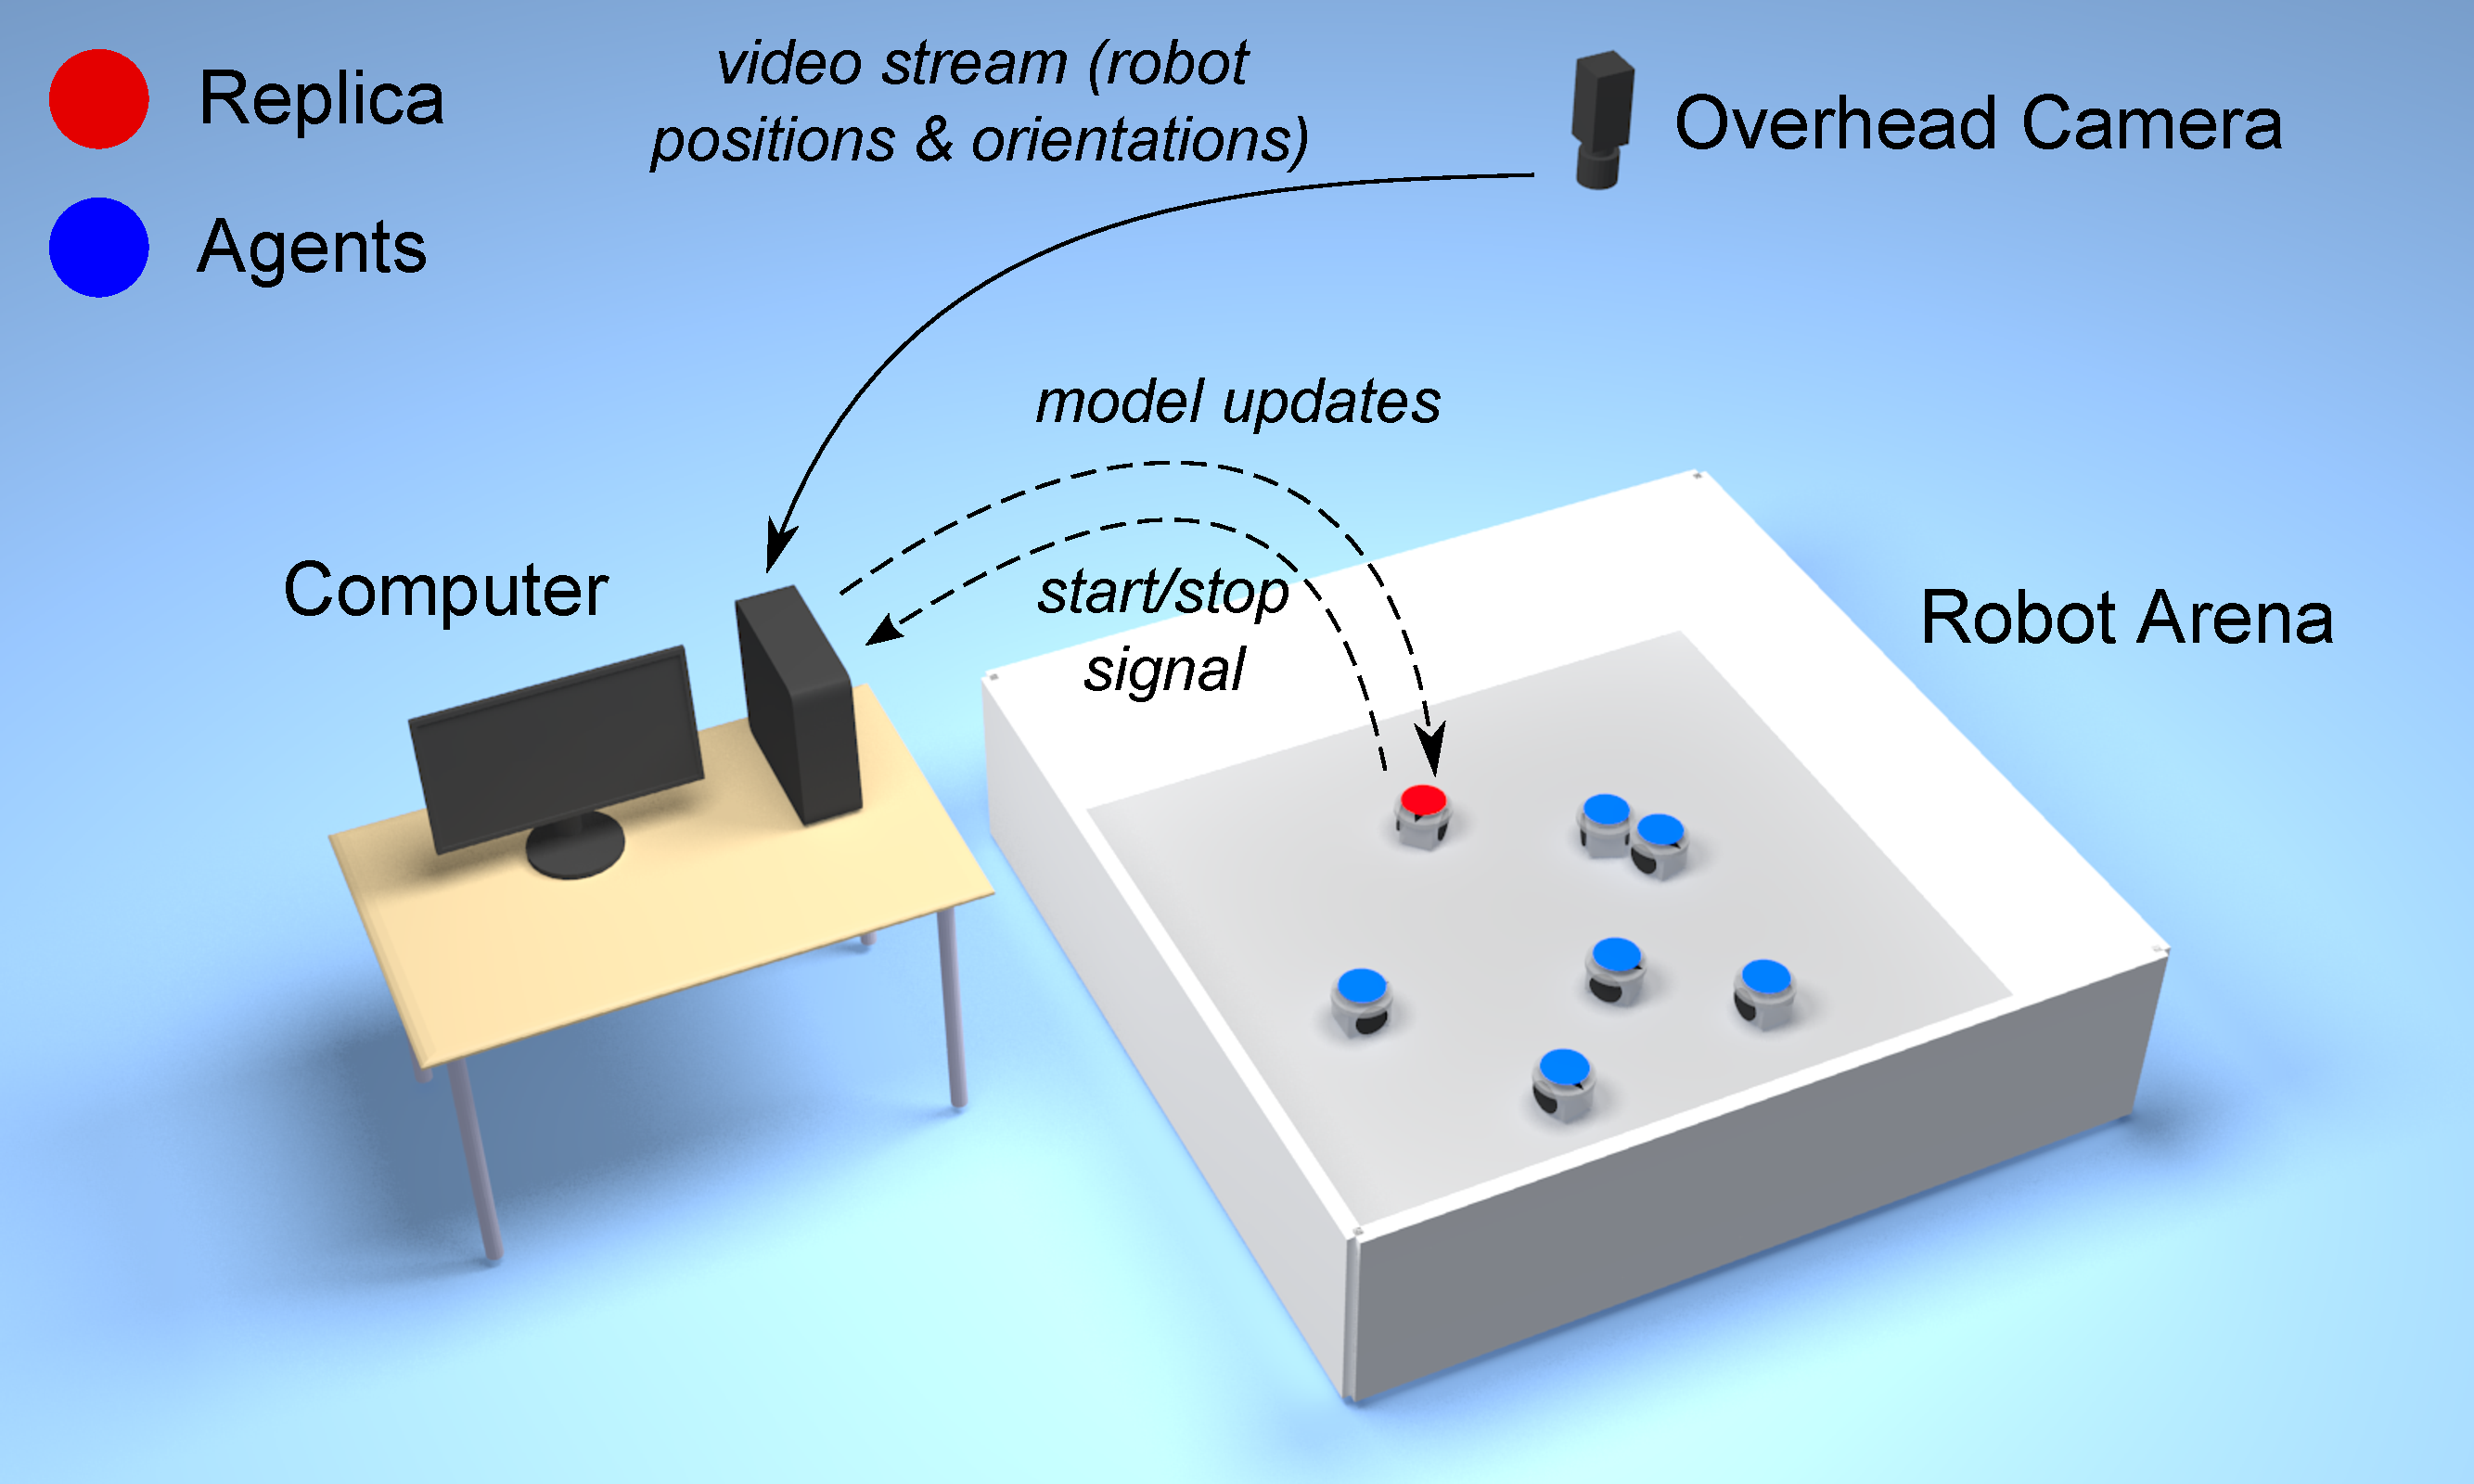
\includegraphics[width=3.5in]{physical_system_setup.pdf}
    \caption{Illustration of the general setup for inferring the behavior of physical agents---e-puck robots (not to scale). The computer runs the coevolutionary algorithm, which produces models and classifiers. The models are uploaded and executed on the replica. The classifiers run on the computer. They are provided with the agents' and replica's motion data, extracted from the video stream of the overhead camera.}
    \label{fig:physical_system_setup}
\end{figure} 

\begin{figure}[!t]
	\centering
	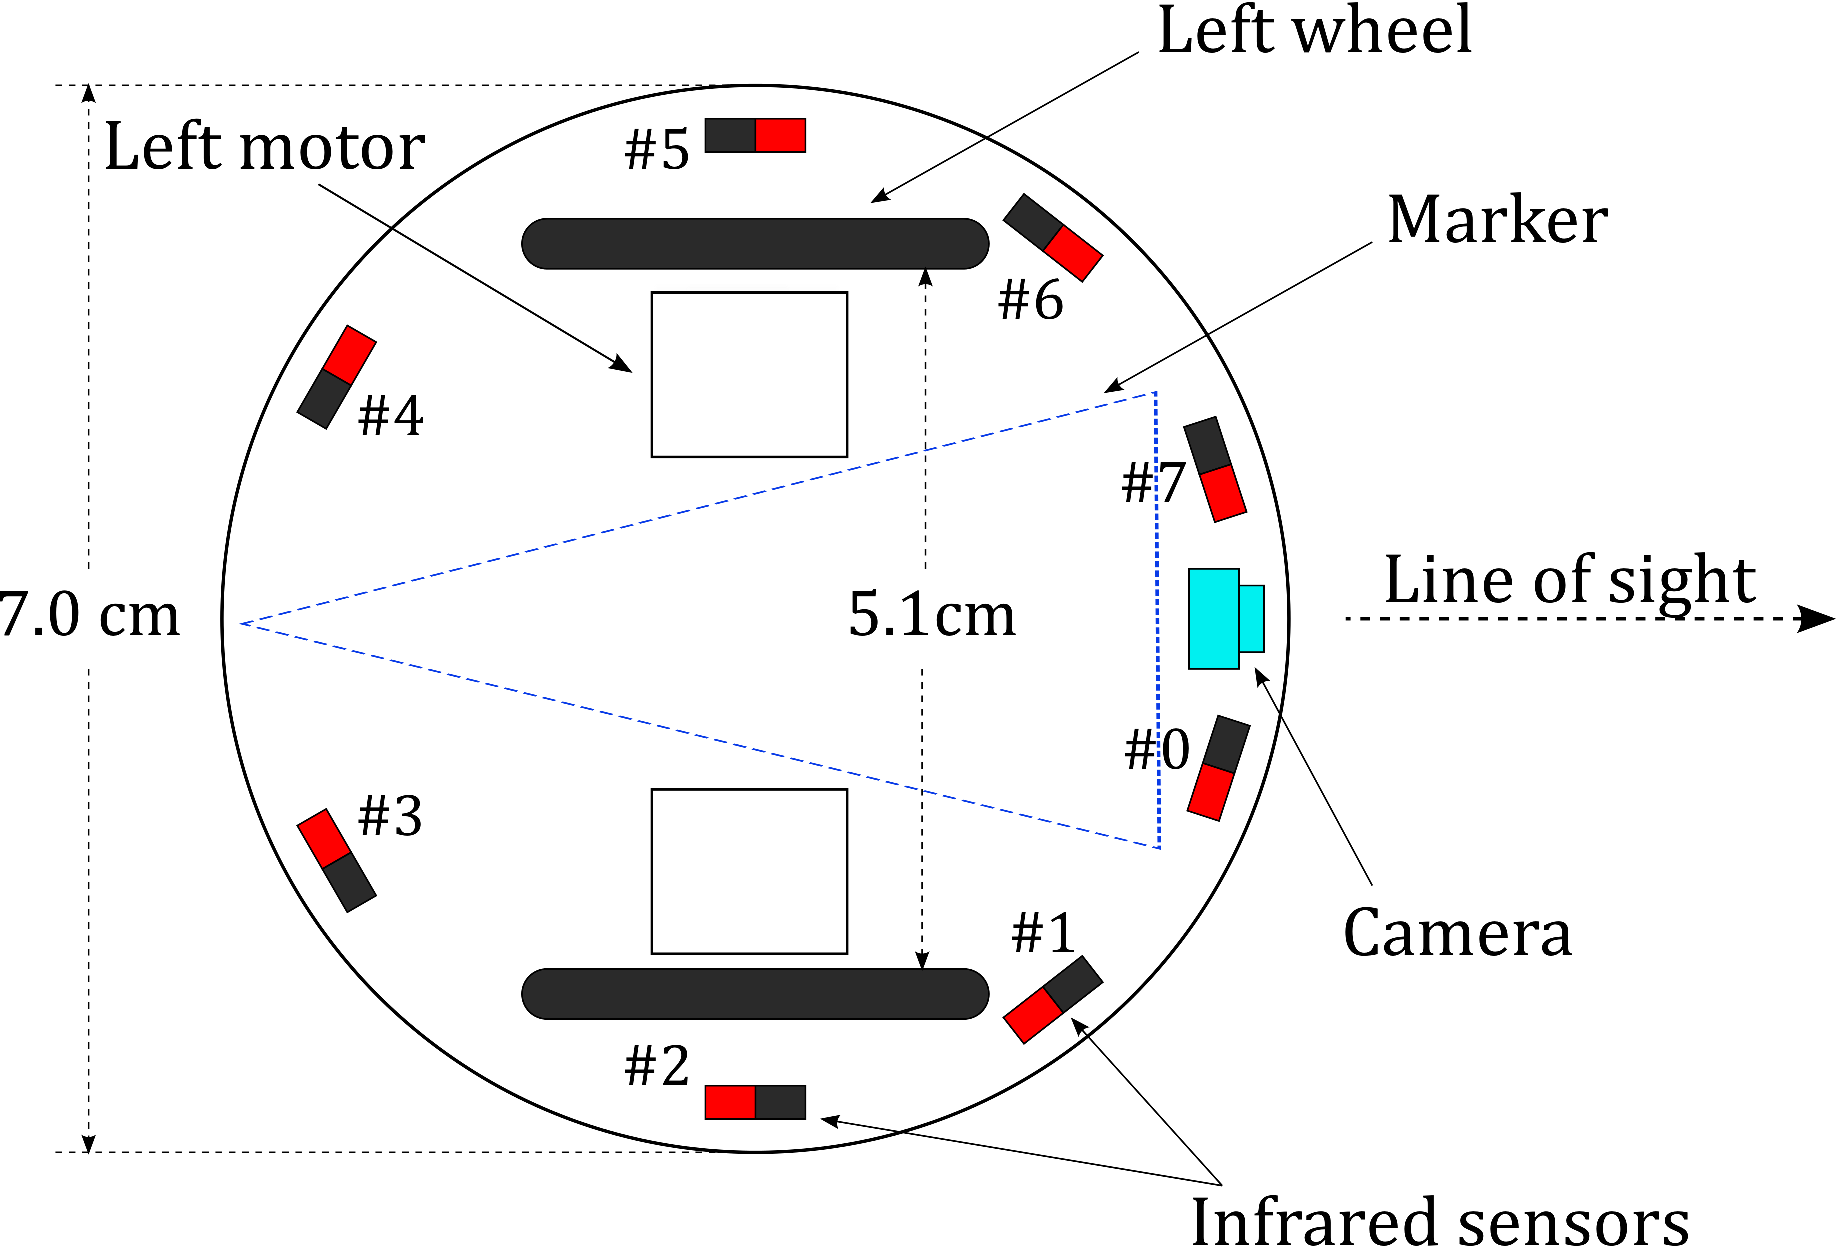
\includegraphics[width=3.5in]{drawing_epuck_schematic.pdf}
	\caption{Schematic top-view of an e-puck, indicating the locations of its motors, wheels, camera and infrared sensors. Note that the marker is pointing towards the robot's back.}
	\label{fig:e_puck_schematic}
\end{figure}

\subsection{Robot Arena}\label{sec:robot_arena_physical_swarm}

The robot arena was rectangular with sides $\unit[200]{cm} \times \unit[225]{cm}$, and bounded by walls $\unit[50]{cm}$ high. The floor had a light gray color, and the walls were painted white.

\subsection{Robot Platform and Sensor Implementations}\label{sec:robot_platform_sensor_implementation}

\subsubsection{Robot Platform}

In Section~\ref{sec:platform_swarm_simulation}, we presented the e-puck's shape and dimensions as a basis for the agents' embodiment in simulation. We now present further details about the e-puck relevant to our physical implementation. A schematic top view of the e-puck, showing the sensors and actuators, is shown in Figure~\ref{fig:e_puck_schematic}.

The e-puck has a on-board micro-controller, which is the Microchip dsPIC30F6014A with 8KB of RAM and 144 KB of flash memory. The two wheels are driven by the stepper motors. The e-puck has a directional (color) camera located in its front. The resolution of the camera is up to $640\times480$, corresponding to the horizontal and vertical angle view of $56\degree$ and $48\degree$. There are eight infrared proximity sensors around the body of the robot. The proximity sensors are only used for collision/wall avoidance in the physical coevolutions where the environment is bounded. 

\subsubsection{Sensor Implementations}

We implemented the line-of-sight sensor using the e-puck's directional camera. For this purpose, we wrapped the robots in black `skirts' (see Figure~\ref{fig:e-puck_body}) to make them distinguishable against the light-colored arena.  However, we use the camera in monochrome mode, and sub-sample the image to $40 \times 15$ pixels, due to the e-puck's limited memory (which cannot even store a single full-resolution image). While in principle the sensor could be implemented using one pixel, we used a column of pixels from a sub-sampled image to compensate for misalignment in the camera's vertical orientation. The gray values from these pixels were used to distinguish robots ($I=1$) against the arena ($I=0$). If any pixel of that column exceeds a certain threshold in its gray scale, the sensor outputs $1$; otherwise, it outputs $0$. For more details about this sensor realization, see~\cite{Gauci2014_ijrr}.

We also used the e-puck's infrared sensors, in two cases. Firstly, before each trial, the robots dispersed themselves within the arena (behavior \textit{R2} in Section~\ref{sec:replica_program_physical_swarm}). In this case, they used the infrared sensors to avoid both robots and walls, making the dispersion process more efficient. Secondly, we observed that using only the line-of-sight sensor can lead to robots becoming stuck against the walls of the arena, hindering the coevolutionary process. We therefore used the infrared sensors for wall avoidance, but in such a way as to not affect inter-robot interactions\footnote{To do so, the e-pucks determine whether a perceived object is a wall or another robot.}. In the following, we details the implementation of these two programs (\textit{disperse} program and~\textit{wall avoidance} program). 

1) The implementation of~\textit{disperse} program after a trial:

After finishing a trial, we disperse the robots for a while (which is equivalent to initial configuration for a new trial) in order to automate the coevolutionary learning process. This program consists of two behaviors ― obstacle avoidance and disperse. The obstacle avoidance behavior is to prevent the robots colliding with other robots and the walls. In particular, before executing the disperse behavior, each robot detects whether some other objects (robots/walls) exist around it using its infrared proximity sensors. If it detects something, it moves away from the objects through adjusting the linear and angular speed accordingly using a single-layer neural network controller. The obstacle avoidance behavior lasts for 3 seconds. In the disperse behavior, each robot is moving forward with a fixed linear speed while avoiding collisions with other robots and the walls. This behavior lasts for 5 seconds.

2) The implementation of~\textit{wall avoidance} program during a trial:

During a trial, in order to reduce the chances of robots getting stuck against the walls (note that the aggregation behavior was designed in an unbounded environment), we imposed a wall avoidance effect to the original behavior, but in such a way as to not affect inter-robot interactions. In particular, when the robot detected the white walls using the infrared sensors or saw another robot (I=1) using the camera, it executed the same behavior. For example, for the agent, it would also turn on the spot when detecting the walls, which makes it easier to avoid the walls. However, the behavior of the replica depends on the model it is executing. Different from the Disperse program, the program of wall avoidance was only triggered when the value of any of the robot's infrared sensor was above a pre-set high threshold. This ensures that the value of the robot's infrared sensors when other robots (covered with a black 'skirt') were nearby was always below the threshold. Therefore, the wall avoidance program did not affect the aggregation of robots.

\section{Motion Capture and Video Processing}\label{motion_capture_and_video_processing_swarm_physical}

\subsection{Motion Capture}\label{sec:motion_capture_swarm_physical}

To facilitate motion data extraction, we fitted robots with markers on their tops, consisting of a colored isosceles triangle on a circular white background. The triangle's color allowed for distinction between robots; we used blue triangles for all agents, and orange and purple triangles for the two replicas. The triangle's shape eased extraction of robots' orientations. Note that the orientation of the triangle is pointing to the backward of the e-puck robot so that it can be easily attached.

The robots' motion was captured using a GigE color camera (Basler Technologies), mounted around $\unit[300]{cm}$ above the arena floor. The camera's frame rate was set to $\unit[10]{fps}$. The video stream was fed to the PC, which performed video processing to extract motion data about individual robots (position and orientation). The size of the arena in the image is $\unit[700]{pixels} \times \unit[800]{pixels}$. An image of the arena captured using the overhead camera is shown in Figure~\ref{fig:robot_arena}.
%
\begin{figure}[!t]
    \centering
    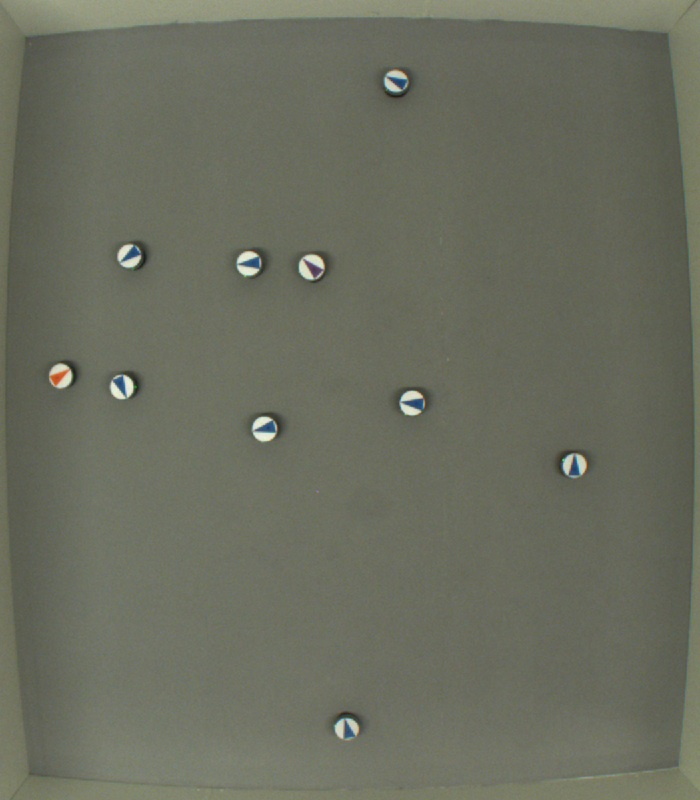
\includegraphics[width=3.0in]{robot_arena.jpg}
    \caption{An image of the robot arena captured by the overhead camera. The robots inside the arena are covered with a colored triangle for facilitating the motion tracking.}
    \label{fig:robot_arena}
\end{figure} 
%
\subsection{Video Processing}\label{sec:video_processing_physical_swarm}

The video processing software was written using OpenCV---an open-source computer vision library~\cite{Gary2008}. The details of the video processing algorithm are described as follows. 

The image captured using the overhead camera was encoded using RGB. We changed the encoding into HSV in order to make the tracking algorithm less sensitive to lighting variation. This was realized using a built-in function inside the OpenCV library. After that, the image was converted into grayscale and thresholded. As the background of the arena was light-colored, there was no need to do background extraction. After that, the color images was converted into binary images. A morphological operation (erosion followed by dilation) is applied on the binary images to filter some noise. Blobs in the binary image with a size above certain threshold (36 pixels) are used for robot detection. These selected blobs indicate the robots in the arena. Figure~\ref{fig:binary_image_individuals} shows the selected blobs in an image. 
%
\begin{figure}[!t]%
	\centering
		\subfloat[Agents\label{fig:binary_agents}]{%
			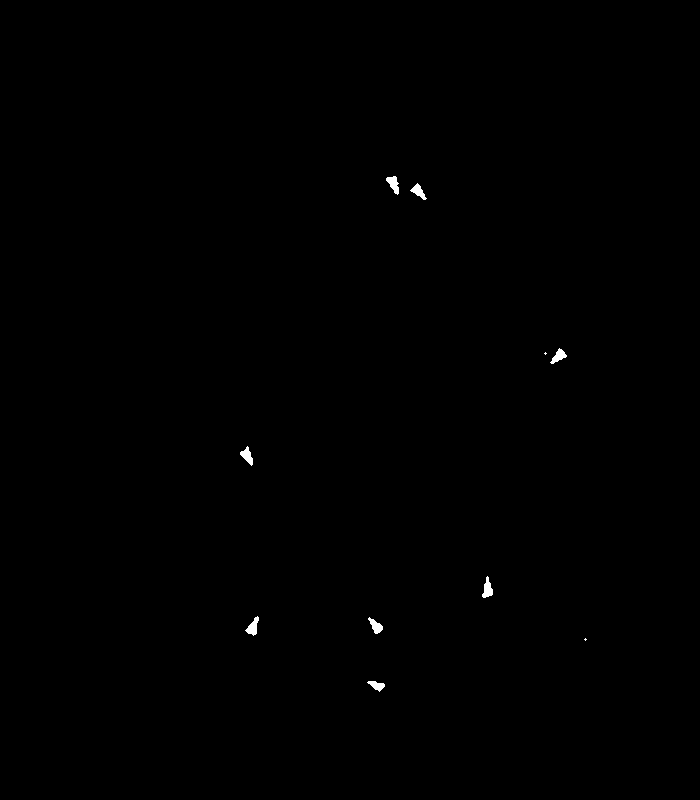
\includegraphics[width=1.65 in]{binary_agents.png} %grid_visualization
		}
		\subfloat[Replica one\label{fig:binary_model_one}]{%
			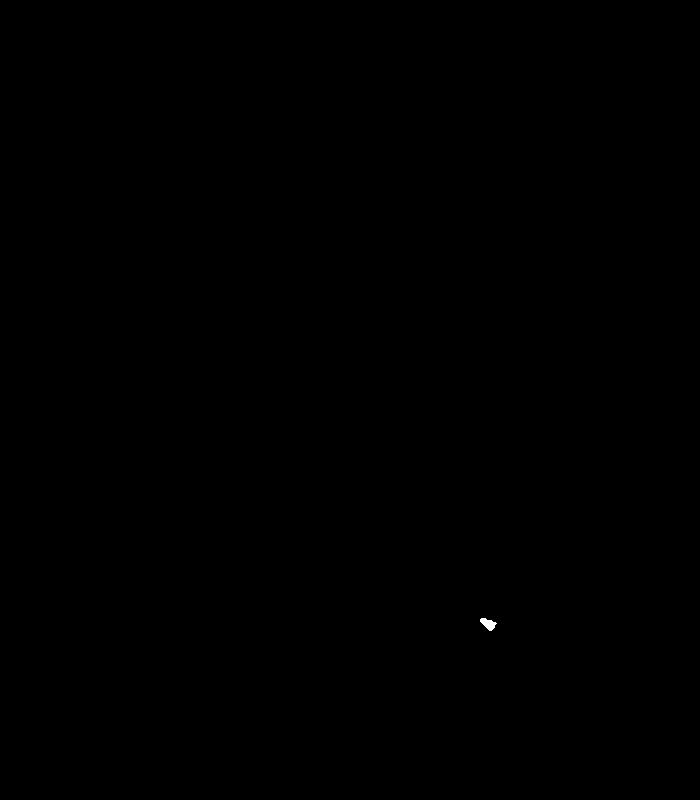
\includegraphics[width=1.65 in]{binary_model_one.png}
		}
		\subfloat[Replica two\label{fig:binary_model_two}]{%
			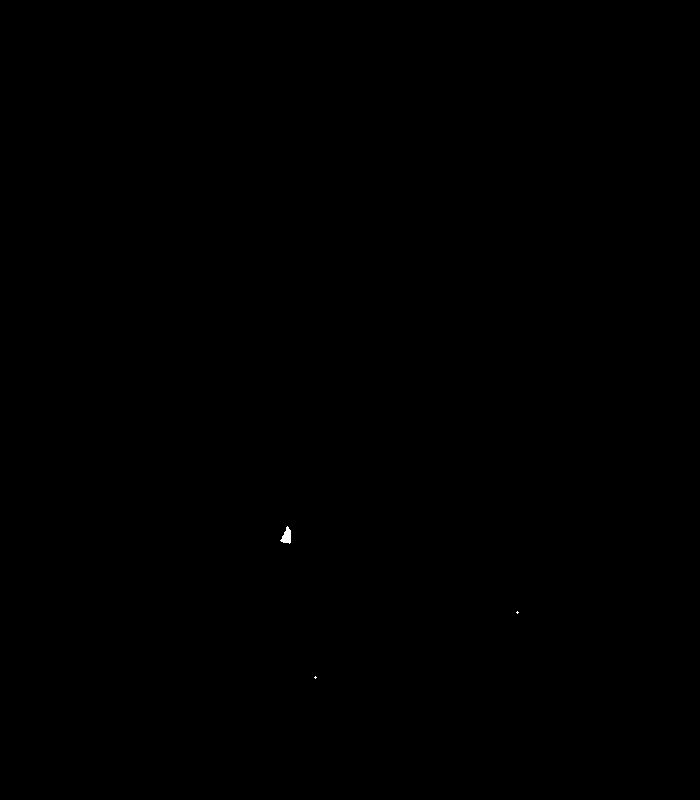
\includegraphics[width=1.65 in]{binary_model_two.png}
		}
		\caption{The binary images showing the blobs of the robots (agents or replicas) in the arena after video processing. The blobs are selected according to certain compactness and size.}
		\label{fig:binary_image_individuals}
\end{figure}
%

The robots were tracked using the nearest neighbor algorithm. For each blob in the image, we found a minimum triangle that encloses the marker, and obtained the coordinates of the three vertices of this triangle. The vertex that has the longest distance to the other two vertices indicates the direction of the robot. Therefore the orientation of the robot was estimated using the vector pointing from the midpoint of the other two vertices to this vertex. We use moments~\citep{Hu1962} to calculate the position of the center of the robot. The x and y coordinate of the position is the $1^\mathrm{th}$ order spatial moments around x-axis and y-axis divided by the $0^\mathrm{th}$ order central moments of the blob, respectively. Figure~\ref{fig:image_processing_flow} shows a diagram of the video processing algorithm. 
%
\begin{figure}[!t]
    \centering
    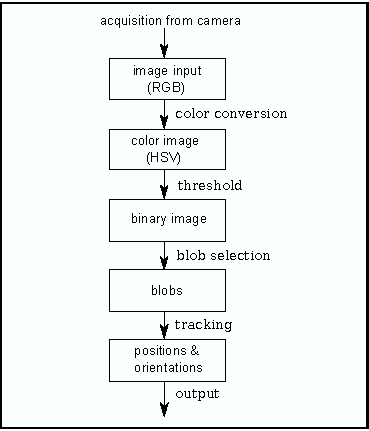
\includegraphics[width=3.5in]{image_processing_flow.pdf}
    \caption{A diagram showing the flow of image processing algorithm used in the tracking system.}
    \label{fig:image_processing_flow}
\end{figure} 
%
%
\begin{figure}[!t]
    \centering
    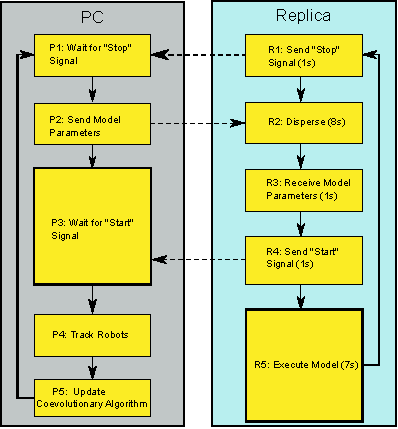
\includegraphics[width=3.5in]{replica_pc_interation.pdf}
    \caption{Schematic of the programs run by the PC and a replica in the physical experiments. Dotted arrows represent communication between the two units. See Section~\ref{sec:coevolution_physical_robots_swarm_physical} for details.}
    \label{fig:agent_pc_interation}
\end{figure} 
%
\section{Coevolution with Physical Robots}\label{sec:coevolution_physical_robots_swarm_physical}

To automate the coevolutionary process, the robots (agents and replicas) were implicitly synchronized. This was realized by making each robot execute a fixed behavioral loop of constant duration. The PC also executed a fixed behavioral loop, but the timing was determined by the signals received from the replicas. Therefore, the PC was synchronized with the swarm. The PC communicated with the replicas via Bluetooth. At the start of a coevolution run, or after a human intervention (see Section~\ref{sec:experimental_setup_swarm_physical}), robots were initially synchronized using an infrared signal from a remote control.

Figure~\ref{fig:agent_pc_interation} shows a flow diagram of the programs run by the PC and the replicas, respectively. Dotted arrows indicate communication between the units. The agents executed a similar behavioral loop to the replicas. In the following, we detail the states of the programs executed by the PC, replicas, and agents.

\subsection{PC Program}

\begin{itemize}
	\item \textit{P1:} \textit{Wait for ``Stop'' Signal.} The program is paused until ``Stop'' signals are received from both replicas. These signals indicate that a trial has finished.
	
	\item \textit{P2:} \textit{Send Model Parameters.} The PC sends new model parameters to the buffer of each replica. % the replicas are still in state \textit{R2}; they are later read by the replicas in state \textit{R3}
	
	\item \textit{P3:} \textit{Wait for ``Start'' Signal.} The program is paused until ``Start'' signals are received from both replicas, indicating that a trial is starting.
	
	\item \textit{P4:} \textit{Track Robots.} The PC waits $\unit[1]{s}$ and then tracks the robots using the overhead camera for $\unit[5]{s}$. The tracking data contains the positions and orientations of the agents and replicas. 
	%During the trial, which lasts $\unit[7]{s}$, the PC tracks the robots using the overhead camera. Potentially misaligned data from the initial and final seconds of this period are discarded. The motion data thus contains the positions and orientations of the agents and replicas over $\unit[5]{s}$. 
	
	\item \textit{P5:} \textit{Update Coevolutionary Algorithm.} The PC uses the motion data from the trial observed in \textit{P4} to update the fitness of the corresponding two models and all classifiers. Once all models in the current generation have been evaluated, the PC also generates new model and classifier populations. The fitness calculation and optimization algorithm are described in Section~\ref{sec:fitness_calculation_swarm}. The PC then goes back to~\textit{P1}. 
\end{itemize}

\subsection{Replica Program}\label{sec:replica_program_physical_swarm}

\begin{itemize}
\item \textit{R1}: \textit{Send ``Stop'' Signal.} After a trial stops, the replica informs the PC by sending a ``Stop'' signal. The replica waits $\unit[1]{s}$ before proceeding with~\textit{R2}, so that all robots remain synchronized. Waiting $\unit[1]{s}$ in other states serves the same purpose. %(agents are programmed to restart $\unit[1]{s}$ after a trial stops)

\item\textit{R2}: \textit{Disperse.} The replica disperses in the environment, while avoiding collisions with other robots and the walls. This behavior lasts $\unit[8]{s}$.

\item\textit{R3}: \textit{Receive Model Parameters.} The replica reads new model parameters from its buffer (sent earlier by the PC). It waits $\unit[1]{s}$ before proceeding with~\textit{R4}.

\item\textit{R4}: \textit{Send ``Start'' Signal.} The replica sends a start signal to the PC to inform it that a trial is about to start. The replica waits $\unit[1]{s}$ before proceeding with~\textit{R5}.

\item\textit{R5}: \textit{Execute Model.} The replica moves within the swarm according to its model. This behavior lasts $\unit[7]{s}$ (the tracking data corresponds to the middle $\unit[5]{s}$, see~\textit{P4}). The replica then goes back to~\textit{R1}.
\end{itemize}

\subsection{Agent Program}

\begin{itemize}
\item The agents follow the same behavioral loops as the replicas. However, in the states analogous to \textit{R1}, \textit{R3}, and \textit{R4}, they simply wait $\unit[1]{s}$ rather than communicate with the PC. In the state corresponding to \textit{R2}, they also execute the \textit{Disperse} behavior. In the state corresponding to \textit{R5}, they execute the original aggregation controller, rather than a model.
\end{itemize}

\section{Experimental Setup}\label{sec:experimental_setup_swarm_physical}

As in simulation, we used a population size of $100$ for classifiers ($\mu = 50$,  $\lambda = 50$). However, the model population size was reduced from $100$ to $20$ ($\mu = 10$,  $\lambda = 10$), to shorten the experimental time. We used $10$ robots: $8$ representing agents executing the original aggregation controller (Equation~\eqref{eq:aggregation_optimal_controller}), and $2$ representing replicas that executed models. This meant that in each trial, $2$ models from the population could be evaluated simultaneously; consequently, each generation consisted of $20/2=10$ trials. 
%Note from the previous section that each trial lasted $\unit[18]{s}$; each generation therefore lasted $10\times 18 = \unit[180]{s}$. We chose to run coevolutions for $100$ generations, for a total time of around $5$ hours per run (excepting human interventions).

The coevolutionary algorithm was implemented without any modification to the code used in simulation (except for model population size and observation time in each trial). We still let the model parameters evolve unboundedly (i.e., in $\mathbb{R}^4$). However, as the speed of the physical robots is naturally bounded, we applied the hyperbolic tangent function ($\tanh{x}$) on each model parameter, before sending a model to a replica. This bounded the parameters to $\left(-1,1\right)^4$, with $-1$ and $1$ representing the maximum backward and forward wheel speeds, respectively.

The coevolution runs proceeded autonomously. In the following cases, however, human intervention was made:
\begin{itemize}
\item The robots had been running continuously for $25$ generations. All batteries were replaced.

\item Hardware failure occurred on a robot, for example because of a lost battery connection or because the robot became stuck on the floor. Appropriate action was taken for the affected robot to restore its functionality.

\item A replica lost its Bluetooth connection with the PC. The connection with both replicas was restarted.

\item A robot indicated a low battery status through its LED after running for only a short time. That robot's battery was changed.
\end{itemize}

After an intervention, the ongoing generation was restarted, to limit the impact on the coevolutionary process.

\begin{figure}[!t]
    \centering
    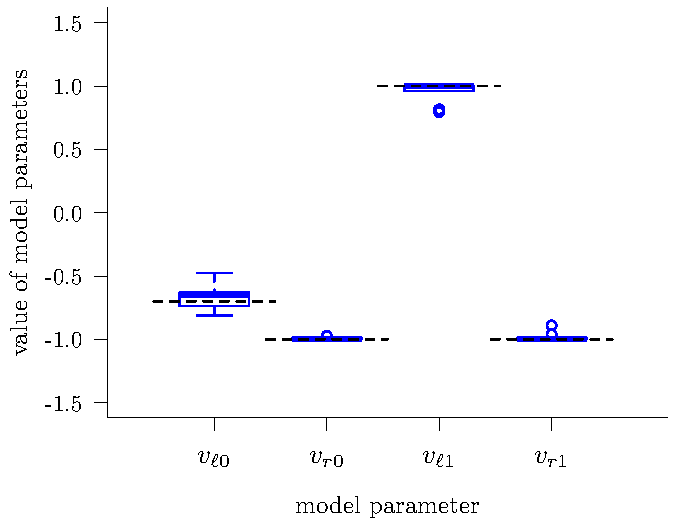
\includegraphics[width=3.5in]{best_model_parameters_physical.pdf}
    \caption{Parameters of the evolved models in the $100^{\textrm{th}}$ generation of $10$ physical coevolution runs. Dotted black lines indicate true values.}
    \label{fig:best_model_parameters_physical}
\end{figure}
%
\section{Results}\label{sec:experimental_results_swarm_physical}

We conducted $10$ coevolution runs using the physical system. Each run lasted $100$ generations, corresponding to $5$ hours (excluding human intervention time). Video recordings of the coevolution runs can be found in the online supplementary materials~\cite{online_supplementary_material_tevc2014}.

\begin{figure}[!t]%
	\centering
		\subfloat[(a) Physical Coevolutions\label{fig:model_parameters_convergence_compare_simulation}]{%
			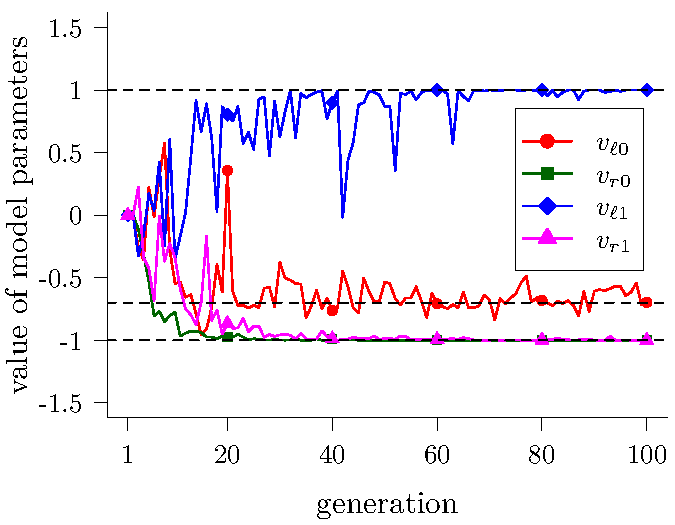
\includegraphics[width=3.5 in]{model_parameters_convergence_compare_physical.pdf} %grid_visualization
		}\\
		\subfloat[(b) Simulated Coevolutions\label{fig:model_parameters_convergence_compare_physical}]{%
			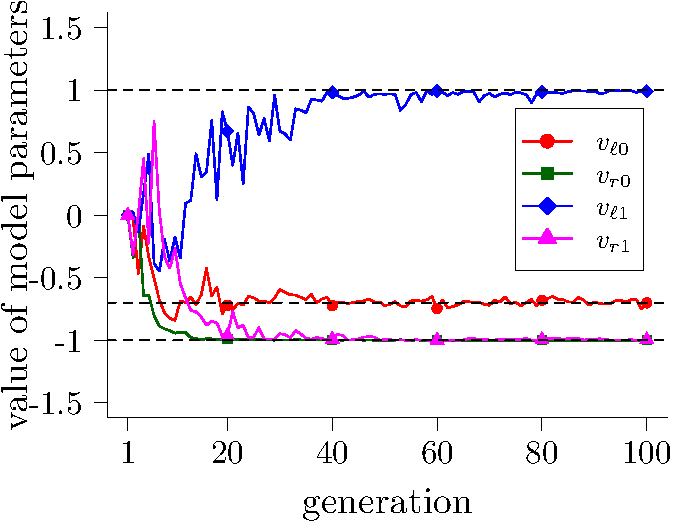
\includegraphics[width=3.5 in]{model_parameters_convergence_compare_simulation.pdf}
		}
		\caption{Evolutionary progress of each model parameter in $10$ (a) physical and (b) simulated coevolution runs. Curves represent median values across $10$ runs. Dotted black lines indicate true values.}
		\label{fig:model_parameters_convergence_compare}
\end{figure}

\subsection{Analysis of Evolved Models}\label{sec:analysis_evolved_model_physical_swarm}

We will first investigate the quality of the models obtained. To select the `best' model from each coevolution run, we post-evaluated all models of the final generation $5$ times using all classifiers of that generation. The parameters of these models are shown in Figure~\ref{fig:best_model_parameters_physical}. The means (standard deviations) of the AEs in each parameter were: $0.08$ ($0.06$), $0.01$ ($0.01$), $0.05$ ($0.08$), and $0.02$ ($0.04$).

To investigate the effects of real-world conditions on the coevolutionary process, we performed $10$ simulated coevolution runs with the same setup as in the physical runs. Figure~\ref{fig:model_parameters_convergence_compare} shows the evolutionary dynamics of the parameters of the evolved models (with the highest subjective fitness) in the physical and simulated coevolution runs. The dynamics show good correspondence. However, the convergence in the physical coevolutions is somewhat less smooth than that in the simulated ones (e.g., see spikes in $v_{\ell 0}$ and $v_{\ell 1}$). 
%One reason for this may be the limitations in motion data capture and extraction. In particular, given the relatively small diameter of the e-puck in our arena, inferring its orientation is particularly challenging.
\begin{figure}[!t]%
	\centering
		\subfloat[(a) Physical Coevolutions\label{fig:MAE_simulation}]{%
			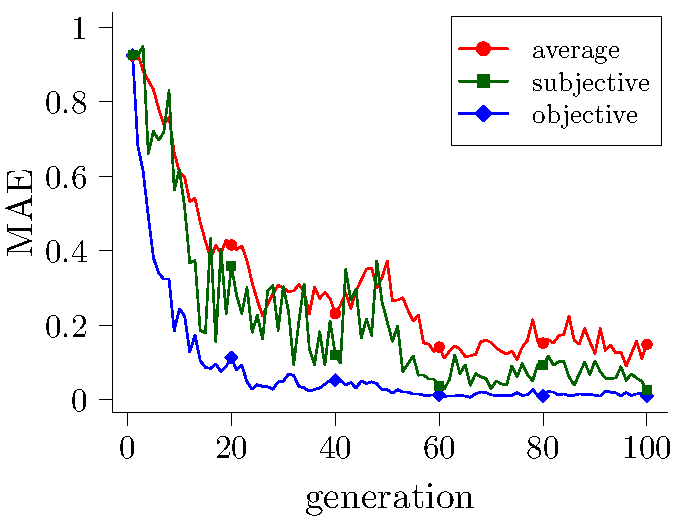
\includegraphics[width=3.5 in]{MAE_physical.pdf} %grid_visualization
		}\\
		\subfloat[(b) Simulated Coevolutions\label{fig:MAE_physical}]{%
			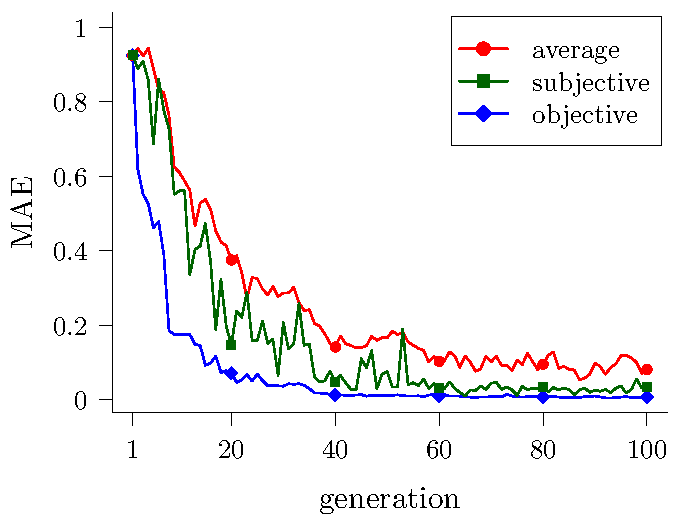
\includegraphics[width=3.5 in]{MAE_simulation.pdf}
		}
		\caption{Evolutionary progress of the MAE (defined in Equation~\eqref{eq:MAE}) of models in $10$ (a) physical and (b) simulated coevolution runs. Curves represent median values across $10$ runs. The red curve represents the average error of all models in a generation. The green and blue curves show, respectively, the errors of the models with the highest subjective and the highest objective fitness in a generation.}
		\label{fig:MAE_compare_simulation_physical}
\end{figure}
In each generation of every coevolution run (physical and simulated), we computed the MAE of each model. We compared the error of the model with the highest subjective fitness with the average and lowest errors. The results are shown in Figure~\ref{fig:MAE_compare_simulation_physical}. For both the physical and simulated coevolution runs, the subjectively best model (green) has an error in between the lowest error (blue) and the average error (red) in the majority of generations. 
%Also in both cases the gap between the error of the subjectively best model and the average error becomes wider as the coevolution proceeds, which means the decision-making ability of the classifiers is improving. This gap, in turn, forces the model population to evolve, as indicated by the downwards trend of the lowest error.
%and only misguided by increasingly good models.

As we argued before (Section~\ref{sec:analysis_evolved_models_swarm_simulation}), in swarm systems, good agreement between local behaviors (e.g., controller parameters) may not guarantee similar global behaviors. For this reason, we performed $20$ trials using $40$ physical e-pucks, lasting $10$ minutes each: $10$ trials with the original controller (Equation~\eqref{eq:aggregation_optimal_controller}), and $10$ trials with a controller obtained from the physical coevolution runs. This latter controller was constructed by taking the median values of the parameters over the $10$ runs, which are:
$$
\mathbf{p}=\left(-0.65, -0.99, 0.99, -0.99\right).
$$
The set of initial configurations of the robots was common to both controllers. As it was not necessary to extract the orientation of the robots, a red circular marker was attached to each robot so that its position can be extracted with higher accuracy in the offline analysis~\cite{Gauci2014_ijrr}.
%
\begin{figure}[!t]%
	\centering
		\subfloat[(a) Largest Cluster Dynamics \label{fig:aggregation_dynamics_proportion}]{
			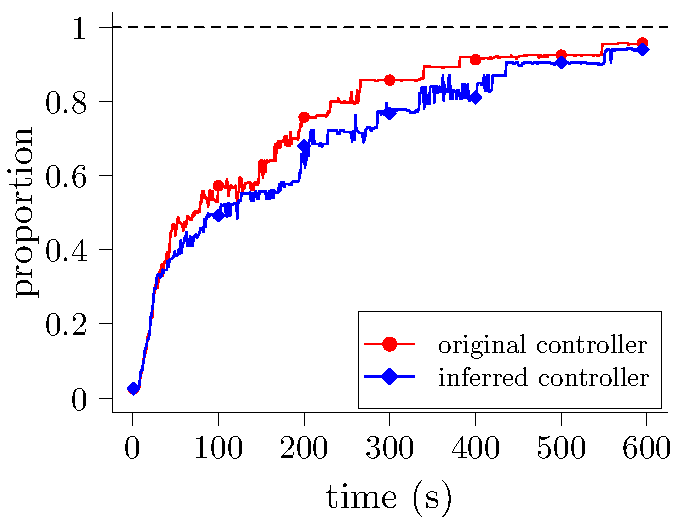
\includegraphics[width=3.5 in]{aggregation_dynamics_proportion.pdf}
		}\\
		\subfloat[(b) Dispersion Dynamics \label{fig:aggregation_dynamics_compactness}]{
			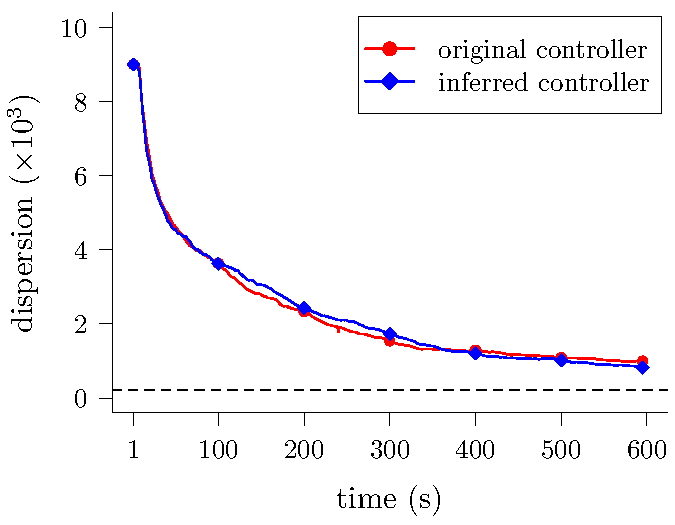
\includegraphics[width=3.5 in]{aggregation_dynamics_compactness.pdf}
		}
		\caption{Average aggregation dynamics in $10$ physical trials with $40$ e-puck robots executing the original controller (red) and the evolved controller (blue). In (a), the vertical axis shows the proportion of robots in the largest cluster; in (b), it shows the robots' dispersion (see Section~\ref{sec:analysis_evolved_models_swarm_simulation}). Dotted lines in (a) and (b), respectively, represent the maximum proportion and minimum dispersion that $40$ robots can achieve.}
		\label{fig:aggregation_dynamics_physical}
\end{figure}
%
Figure~\subref*{fig:aggregation_dynamics_proportion} shows the proportion of robots in the largest cluster\footnote{A cluster of robots is defined as a maximal connected subgraph of the graph defined by the robots' positions, where two robots are considered to be adjacent if another robot cannot fit between them~\cite{Gauci2014_ijrr}.} over time with the original and inferred controllers. Figure~\subref*{fig:aggregation_dynamics_compactness} shows the dispersion (as defined in Section~\ref{sec:analysis_evolved_models_swarm_simulation}) of the robots over time with the two controllers. The aggregation dynamics of the original and inferred behaviors show good correspondence. Figure~\ref{fig:aggregation_snapshoot_physical_validation} shows a sequence of snapshots from a trial with $40$ e-pucks executing the evolved controller.

We also performed a scalability study in simulation to compare the real and evolved controllers. We calculated the time taken to form a single cluster with different numbers of robots: $n \in \lbrace10, 20, \dots, 100\rbrace$. For each number of robots, we performed $30$ trials with each controller. The results are shown in Figure~\ref{fig:aggregation_model_validation_physical}. In all cases, the real controller slightly outperforms the evolved one.
However, with either controller, the robots aggregate in a relatively short time ($<\unit[600]{s}$). There is a statically significant difference in aggregation times with the two controllers for $n= 10, 30, 50, 70, 80, 90$---but this suggests no particular pattern with respect to $n$. We also performed a linear least squares regression on the aggregation times with the two controllers. The fits were: $T = 53.2 + 2.2n$ for the real controller, and $T = 64 + 2.4n$ for the evolved controller ($n>1$). This indicates that the evolved controller does not scale much worse than the real one.

\begin{figure}[!t]
	\centering
	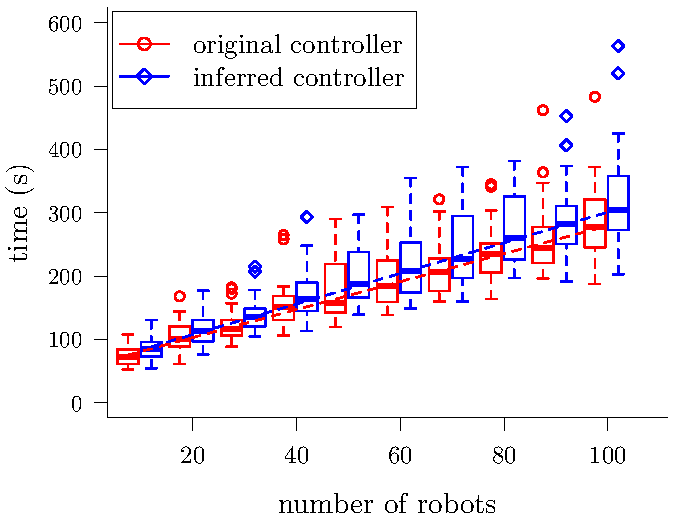
\includegraphics[width=3.5in]{aggregation_model_validation_physical.pdf}
	\caption{Time taken for different numbers of robots to aggregate into a single cluster. Each box corresponds to $30$ 			    simulation trials with the real controller (red), and the controller obtained from the physical coevolution runs (blue).}
	\label{fig:aggregation_model_validation_physical}
\end{figure}

\captionsetup[subfigure]{labelformat=empty}  
\begin{figure*}[!t]
	\centering
	\subfloat[initial configuration]{
		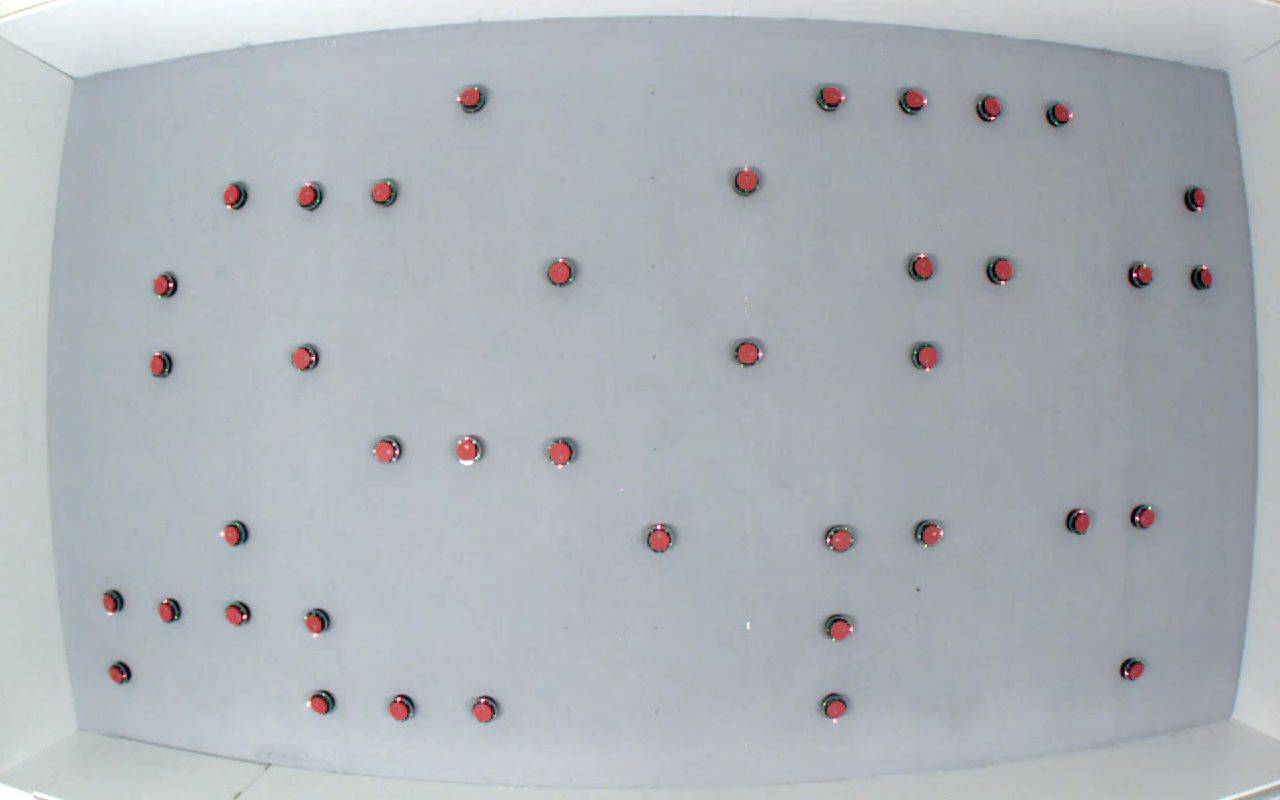
\includegraphics[width = 1.7 in]{physical_snapshot_0s.jpg}
	}
	\subfloat[after $20$ $\unit{s}$]{
		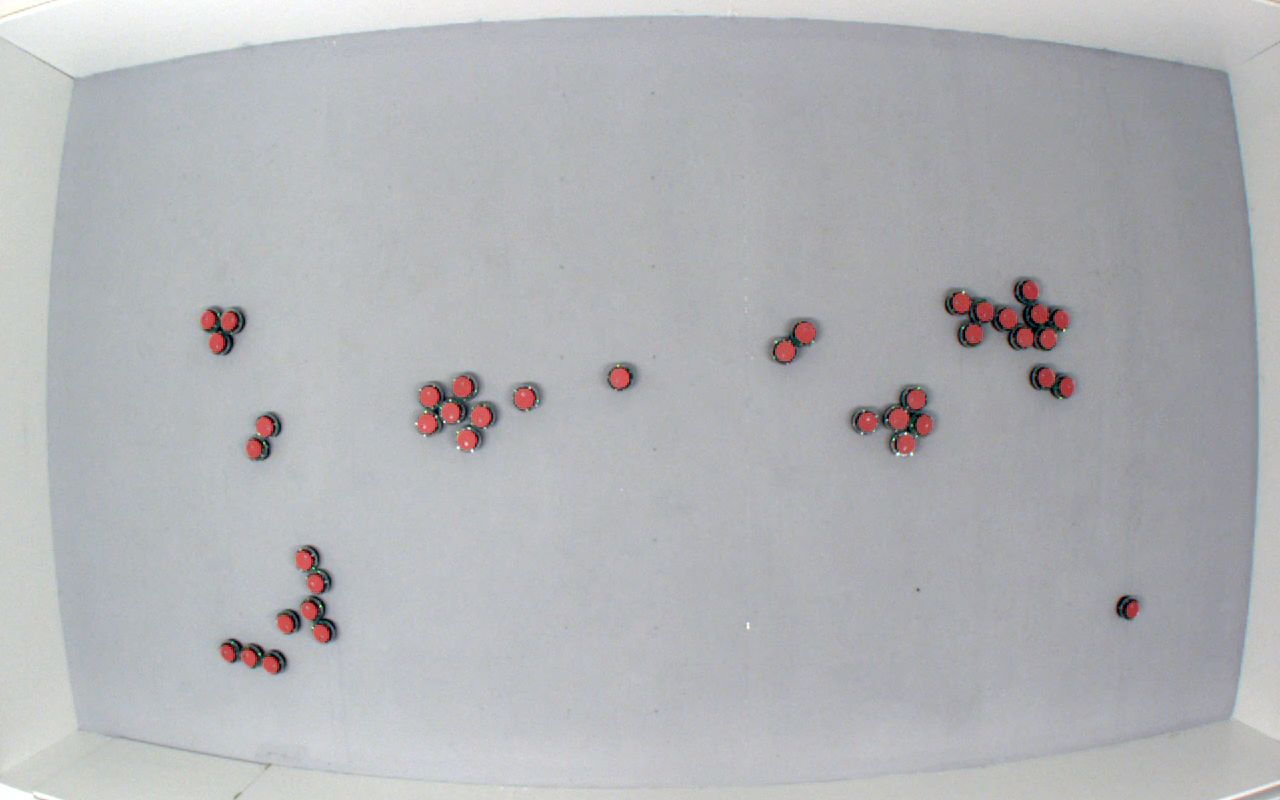
\includegraphics[width = 1.7 in]{physical_snapshot_20s.jpg}
	}\\
	\subfloat[after $40$ $\unit{s}$]{
		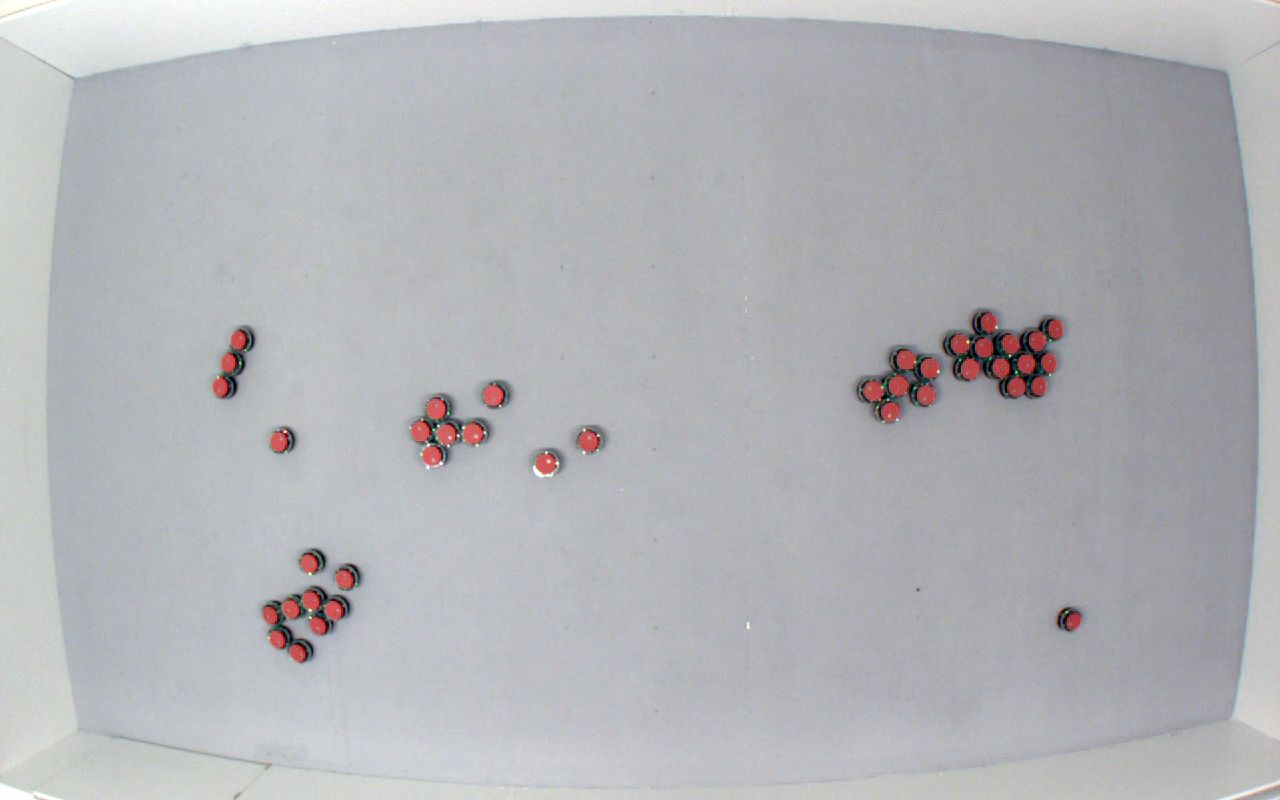
\includegraphics[width = 1.7 in]{physical_snapshot_40s.jpg}
	}
	\subfloat[after $180$ $\unit{s}$]{
		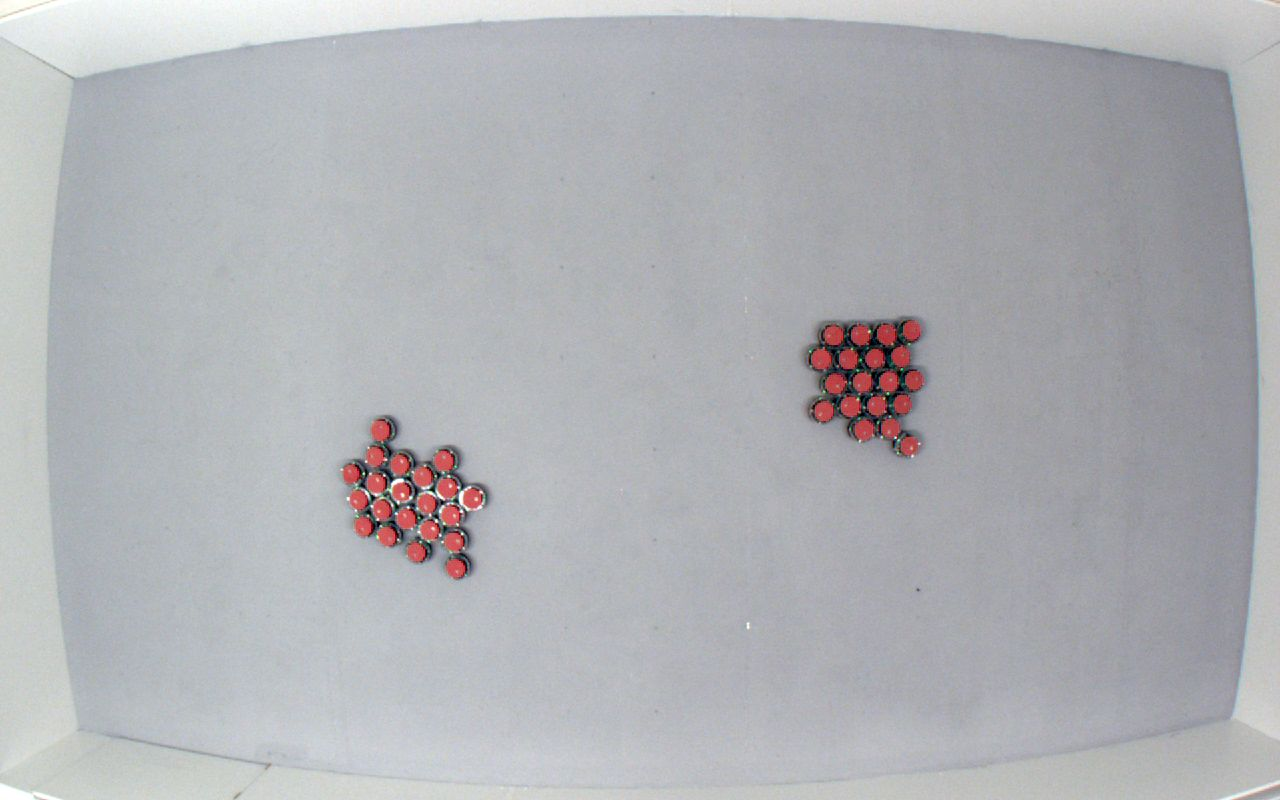
\includegraphics[width = 1.7 in]{physical_snapshot_180s.jpg}
	}\\
		\subfloat[after $360$ $\unit{s}$]{
		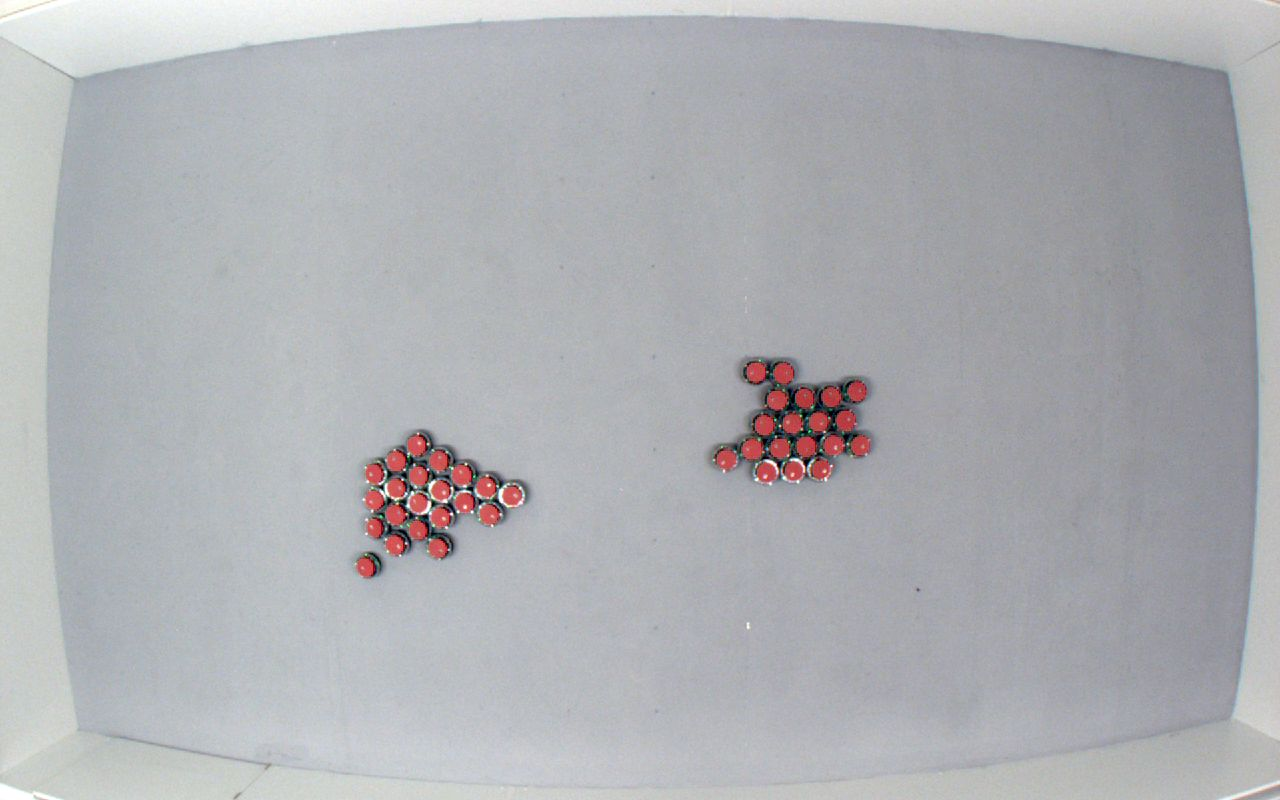
\includegraphics[width = 1.7 in]{physical_snapshot_360s.jpg}
	}
	\subfloat[after $420$ $\unit{s}$]{
		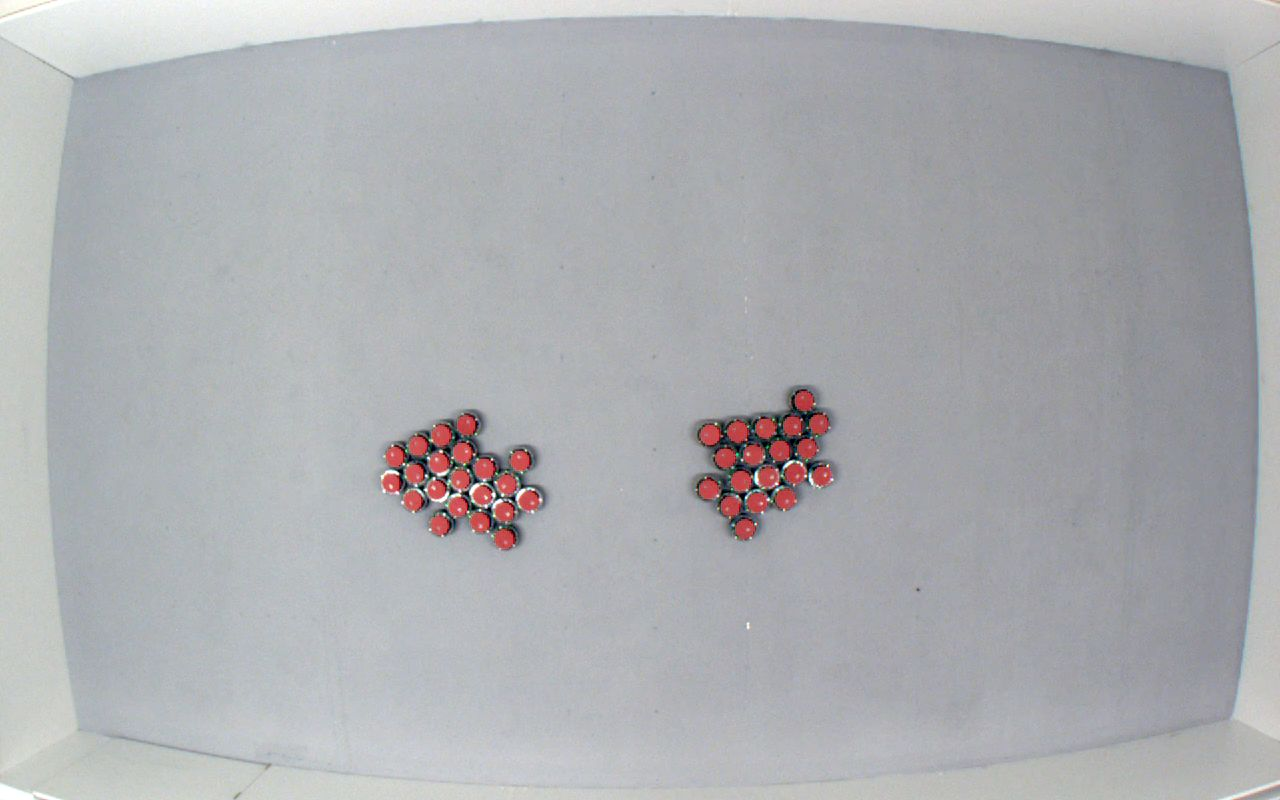
\includegraphics[width = 1.7 in]{physical_snapshot_420s.jpg}
	}\\
	\subfloat[after $480$ $\unit{s}$]{
		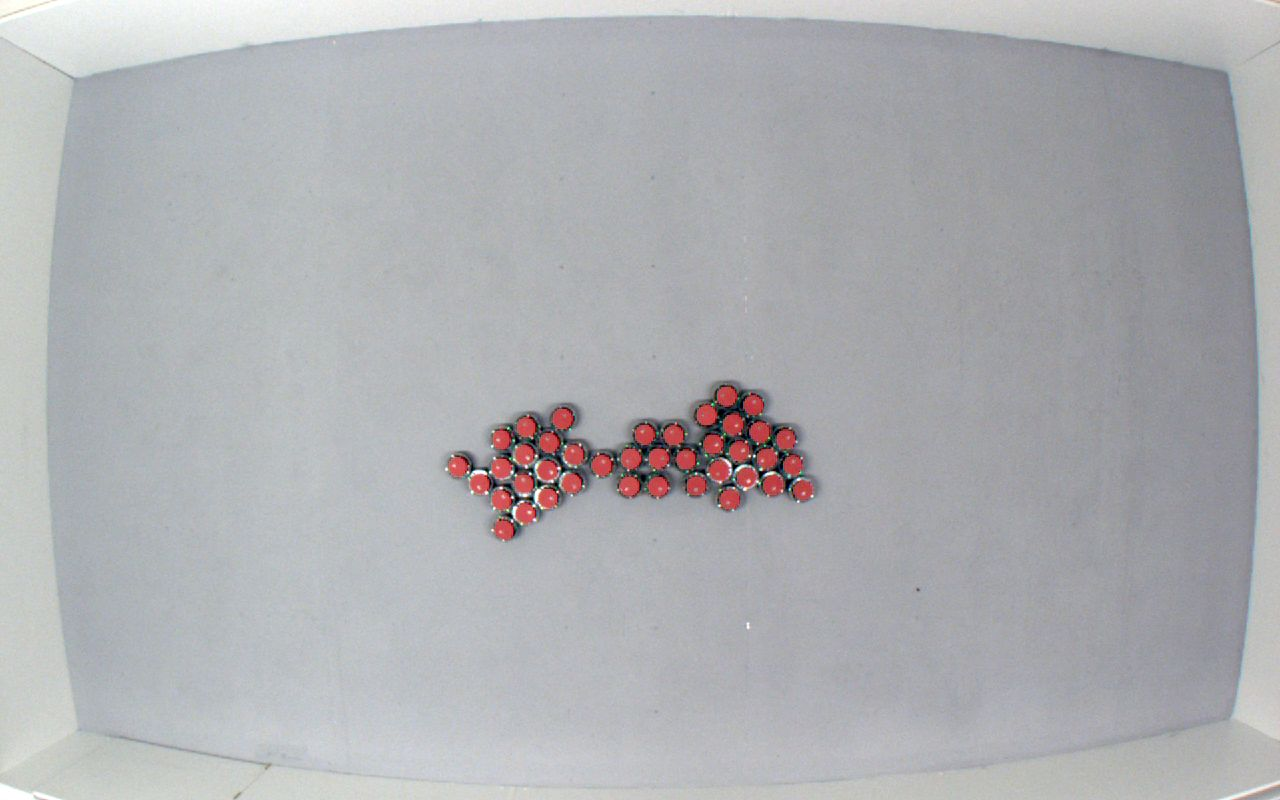
\includegraphics[width = 1.7 in]{physical_snapshot_480s.jpg}
	}
	\subfloat[after $600$ $\unit{s}$]{
		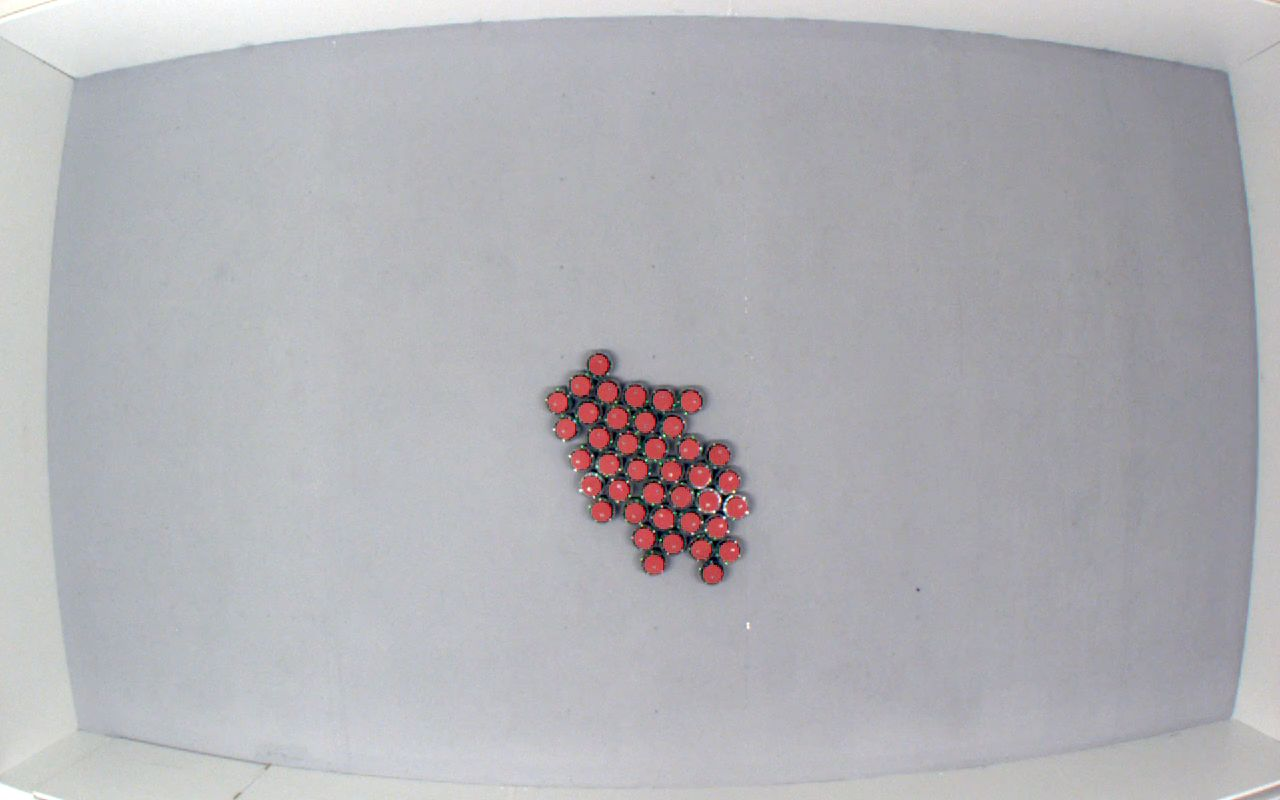
\includegraphics[width = 1.7 in]{physical_snapshot_600s.jpg}
	}
	\caption{Example of a collective behavior obtained by \textit{Turing Learning}. A group of $40$ e-puck robots, each executing the inferred model, aggregates in a single spot.}%The behavior was automatically learned through observation of swarms of physical robots.
	\label{fig:aggregation_snapshoot_physical_validation}
\end{figure*}

A video accompanying this paper shows the evolutionary process of the models (in a particular coevolution run) both in simulation and on the physical system. Additionally, videos of all $20$ post-evaluation trials with $40$ e-pucks, are available in~\cite{online_supplementary_material_tevc2014}.

\subsection{Analysis of Evolved Classifiers}\label{sec:analysis_evolved_classifier_physical_swarm}
%\textcolor{red}{We will now investigate the classifiers' performance. First, we investigate whether the the classifiers' ability of making judgment improves over generations. This could be reflected by comparing the difference between the model with the highest subjective (selected by the classifiers) and the model with the highest objective fitness (the one with the least square error).} As we discussed in Section~\ref{sec:analysis_of_evolved_classifiers_simulation}, the classifier systems obtained in simulation have a good decision accuracy.

When post-evaluating the classifiers evolved in the physical coevolution runs, we limited the number of candidate models to $100$, in order to reduce the experimental time. Each candidate model was randomly chosen with uniform distribution from $[-1,1]^4$. Figure~\ref{fig:classifier_decision_accuracy_physical} shows the average decision accuracy of the best classifiers and classifier systems over the $10$ coevolution runs. Similar to the results in simulation, the classifier systems obtained in the physical coevolution runs still have a high decision accuracy. The \textit{classifier system (archive)} has a higher accuracy than that of the \textit{classifier system (subjective)} and \textit{best classifier (objective)}. However, in contrast to simulation, the decision accuracy of the \textit{best classifier (subjective)} and \textit{best classifier (archive)} does not drop within $100$ generations. This could be due to the smaller model population size in the physical coevolution runs, which may have prevented the classifiers from getting over-specialized in a short time. 
%To see if we can still get an accurate classifier system in physical experiments, we did the same evaluation. However, as performing a grid search took so much time, we only evaluated the classifiers using a limited number of candidates. 
% Figure~\subref*{fig:model_parameters_convergence_compare_physical}, the error of the models with the highest objective fitness is becoming smaller until about $60^\textrm{th}$ generation, and then it increases slightly. We suspect that this is due to the fact that when the replica behaves more like the agents (that is, the model parameters converge to their real value), it is more likely to collide with them (i.e., to aggregate). the chance of its collision with other agents is higher than those replicas that executes `worse' models.

To investigate whether the decision accuracy is still a good measurement of the quality of the classifiers in the physical coevolution runs, we plot a figure showing the fitness of the best classifiers corresponding to Figure~\ref{fig:classifier_decision_accuracy_physical}. The fitness is calculated based on the $100$ randomly generated models. The results are shown in Figure~\ref{fig:classifier_fitness_physical}. Similar to the results obtained in simulation, the trend of fitness curves show good correspondence to that of the decision accuracy in Figure~\ref{fig:classifier_decision_accuracy_physical}. The gap between the~\textit{best classifier (decision)} and~\textit{best classifier (objective)} in the physical experiments is bigger than that in simulation. One reason for this may be the limitations in motion data capture and extraction. Note that given the relatively small diameter of the e-puck in our arena, inferring its orientation is particularly challenging.

\begin{figure}[!t]
\centering
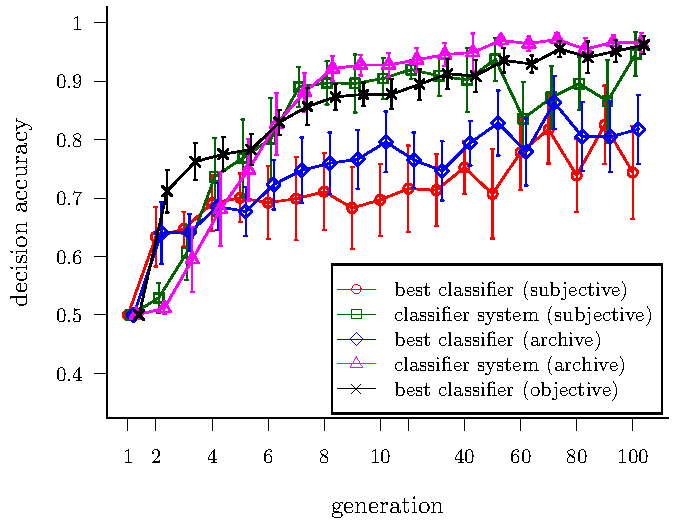
\includegraphics[width=3.5in]{classifier_decision_accuracy_physical.pdf}
\caption{The average decision accuracy of the best classifiers and classifier systems over generations (nonlinear scale) in $10$ physical coevolution runs. The error bars show standard deviations. See text for details.}
\label{fig:classifier_decision_accuracy_physical}
\end{figure}

\begin{figure}[!t]
	\centering
	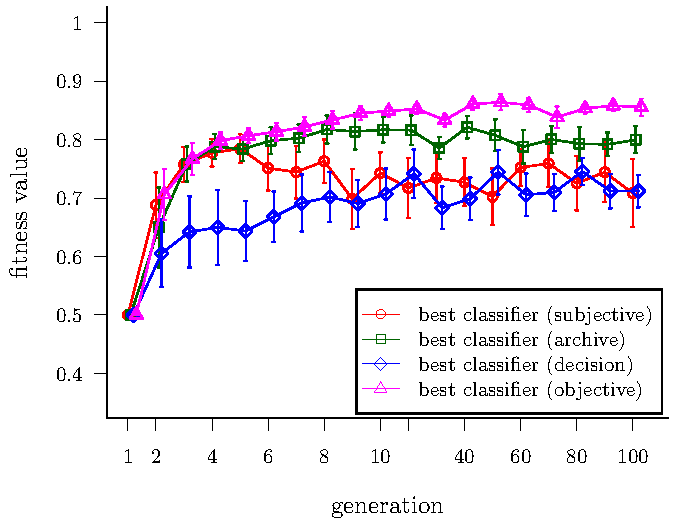
\includegraphics[width=3.5 in]{classifier_fitness_physical.pdf}
	\caption{This plot shows the average fitness of the classifiers over generations (nonlinear scale) in $10$ physical coevolution runs. The fitness is calculated based on $100$ randomly generated models. See text for details.}
	\label{fig:classifier_fitness_physical}
\end{figure}

\begin{figure}[!t]
    \centering
    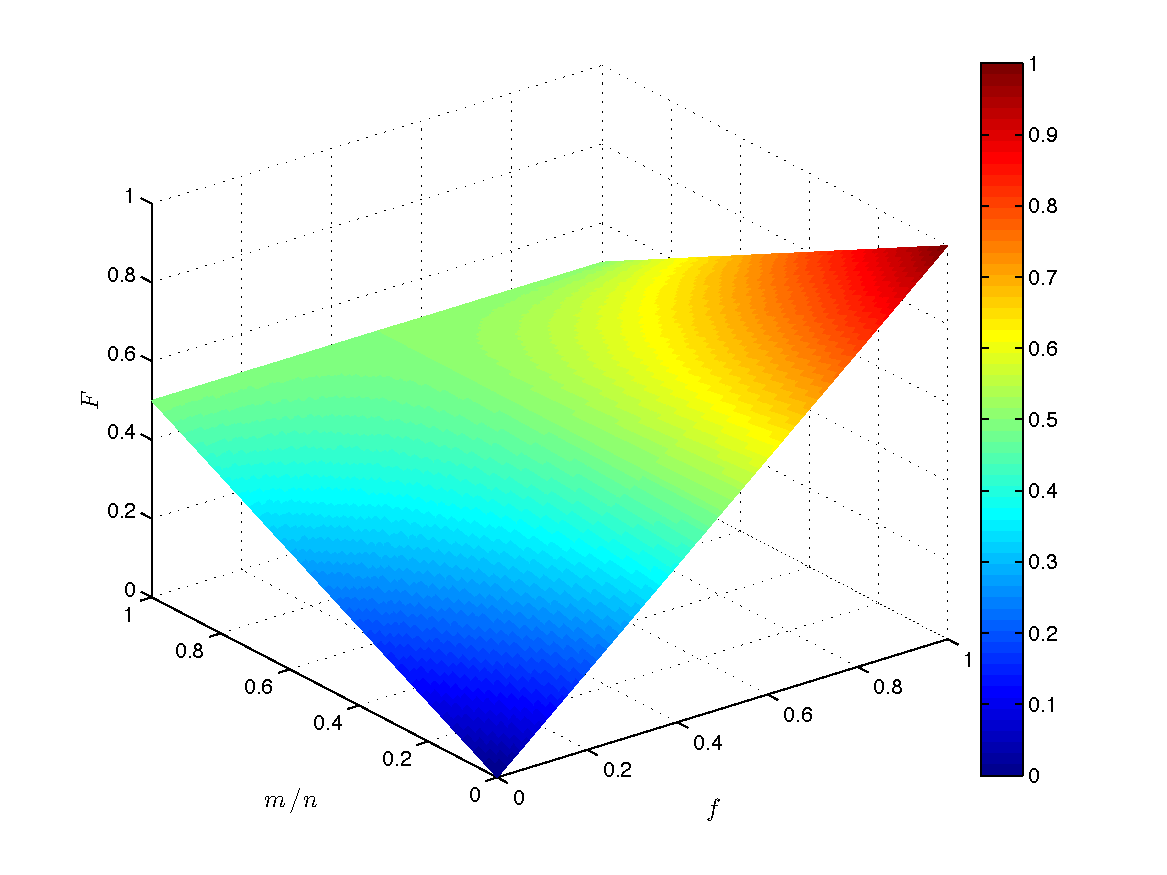
\includegraphics[width=3.5in]{algorithm_sensitivity_analysis.pdf}
    \caption{This plot shows the relationship between the old fitness, $f$, and the new fitness, $F$, of the classifiers, when the failure ratio of agents in the swarm, $\frac{m}{N}$, changes. When $m = 0$ or $N \rightarrow \infty$, $F=f$. When $0 < \frac{m}{N} < 1$, $F$ is shifted, but the fitness order is not changed.}
    \label{fig:analysis_algorithm}
\end{figure}

\section{Analysis of Sensitivity for Individual Failure}\label{sec:analysis_algorithm}

In the physical experiments, we have observed that some robots may get stuck or stop working because of the reasons mentioned in Section~\ref{sec:experimental_setup_swarm_physical}. This could also happen in a real swarm system, for example, some individuals may stop moving or display other abnormal behaviors due to various factors such as collision. These abnormal behaviors (which are considered failure here) may not be recognized during the process of experiments. Therefore, we have analyzed whether abnormal behaviors (failure) of some individuals may bias the evolution and hence affect performance of our proposed coevolutionary approach. Assuming the failure is equally likely to be present in the replica and agent in a trial. We have proved that: \textbf{\textit{Turing Learning} is not biased by failure of certain individuals in the swarm.} The mathematical proof is provided as follows:
 
\begin{proof}
Let $n$ be the total size of the group, consisting of $n-1$ agents and $1$ replica. $m$ represents the number of individuals that fail ($m<n$) in a trial. $p$ and $q$ are the probabilities of a classifier to make the correct judgment for models and agents respectively. Therefore, the expected fitness of the classifier without failure of any individuals in one generation, $f_c$, is equal to $\frac{p+q}{2}$. $f_m$ denotes the fitness of a model in that generation. 

There are two failure cases: 1) failure with the replica; 2) failure without the replica. We assume that if an individual fails during a trial, the classifier makes random judgment, that is, it has equal probability, which is $50\%$, of judging the individual as an agent or a model. If failure exists in a trial, the probability that failure with the replica occurs, $p_1$, is as follows:
\begin{equation}
{p_1} = {\binom{n-1}{m-1}} / {\binom{n}{m}} = \frac{m}{n}.
\end{equation}
The probability that failure without the replica occurs in a trial, $p_2$, is: $1 - p_1 = \frac{n-m}{n}$. The proof is divided into two parts: one for the classifiers and the other is for models.

For the classifier, the new fitness in the first failure case, $f_{c1}$, can be calculated as follows:
\begin{equation}\label{equ:f1:classifier}
{f_{c1}} = p_1 \cdot (\frac{1}{2} + \frac{1}{2} \cdot \frac{m-1}{n-1} + \frac{q \cdot (n-m)}{n-1}) /2.
\end{equation}
In the second failure case, the new fitness of the classifier, $f_{c2}$, is given by:
\begin{equation}\label{equ:f2:classifier}
{f_{c2}} = p_2 \cdot (p + \frac{1}{2} \cdot \frac{m}{n-1} + \frac{q \cdot (n-m-1)}{n-1}) / 2.
\end{equation}
Combining Eqs.~\eqref{equ:f1:classifier} and~\eqref{equ:f2:classifier} and simplifying the resulting expression, the new fitness, $F_c$, of the classifier when $m$ individuals fail in a trial is:
\begin{equation}\label{equ:F:classifier}
{F_c} = f_{c1} + f_{c2} = f_c \cdot (1-\frac{m}{n}) + \frac{m}{2n}.
\end{equation}

In Equation\eqref{equ:F:classifier}, $F_c$ is monotonic increasing in terms of $f_c$. When $f_c$, is equal to $0.5$, $F_c$ maintains the same value. When $f_c$ is greater than (or smaller than) $0.5$, $F_c$ is decreased (or increased) but still greater (or smaller) than $0.5$. Therefore, the fitness order of all the classifiers after failure of $m$ individuals in a trial is not changed, which means it does not affect the selection of the classifiers in the evolutionary process. 
%http://www.numberempire.com/simplifyexpression.php Figure~\ref{fig:analysis_algorithm} visualized how the fitness of the classifiers is shifted when failure of agents occurs. %{F_c} = f_{c1} + f_{c2} = \frac{m}{2N}[1 + (p + q) \cdot \frac{N-m}{m}] = f \cdot (1-\frac{m}{N}) + \frac{m}{2N}.

For the model, it has a new fitness of $f_{m1} = \frac{m}{n} \cdot \frac{1}{2}$ and $f_{m2} = \frac{(n-m) \cdot f_m}{n}$ in the first and second failure case, respectively. Therefore, the new fitness of the model, $F_m$, when $m$ individuals fail in a trial is:
\begin{equation}\label{equ:F:model}
{F_m} = f_{m1} + f_{m2} = f_m \cdot (1-\frac{m}{n}) + \frac{m}{2n}.
\end{equation}
Comparing Eqs.~\eqref{equ:F:classifier} and~\eqref{equ:F:model}, we can see that the fitness order of all the models is also unchanged when failure occurs in a trial.
\end{proof}

\section{Summary}\label{sec:summary_swarm_physical}

%In this chapter, we presented a physical autonomous coevolutionary system for identifying the aggregation behavior in Chapter~\ref{ch:swarm_simulation} using swarms of e-puck robots. The behavior was learned successfully, and the results obtained in the physical experiments show good correspondence to those obtained in simulation. This showed the robustness of our metric-free coevolutionary method with respect to noise and uncertainties in real world, which provided a first step towards automated reversing engineering of  swarm behaviors with little human intervention~\cite{King2009, Schmidt2009}. 

In this chapter, the~\textit{Turing Learning} method was validated using a physical autonomous coevolutionary system. We applied it to identify the aggregation behavior in swarms of e-puck robots. The behavior was learned successfully, and the results obtained in the physical experiments showed good correspondence to those obtained in simulation. This shows the robustness of our method with respect to noise and uncertainties in real world. \textit{Turing Learning} could be beneficial in the context of science automation~\cite{King2009, Schmidt2009}, in particular to reveal the mechanisms underpinning collective animal behavior.

The model obtained in the physical coevolution runs was validated using $40$ e-puck robots. The global behavior of the obtained model is similar to that of the original controller. The selected classifier system over the coevolution runs still obtained a high performance, which means our classifier system could be potentially applied to detect or monitor the behaviors of the agents in a swarm. 
% The step of validation is necessary in our approach. As the classifiers only observed the motion of each individual, and were not provide any information about the global behaviors of the agents. One case that could happen is the evolved model parameters are similar to those of the agents, but the global behaviors of the models and agents are different. 

In order to speed up the coevolutionary process, different from simulation, we used two replicas instead of one. Therefore, two models can be executed simultaneously. In principle, we could further speed up the process through using more replicas in parallel. However, considering the reliability of communication between the replicas and PC as well as the influence of replicas on the whole swarm behaviors, a limited number of replicas is recommended. 

We have proved that \textit{Turing Learning} is robust to failure of individuals in the mixed group. That is, even if some individuals fail during the trials, it won't bias the models obtained. This is another advantage of our \textit{Turing Learning} method, as other metric-based system identification approaches may be biased due to the abnormal behavior of even a single agent.

